\documentclass[11pt,a4paper]{article}

\usepackage[utf8]{inputenc}
\usepackage[T1]{fontenc}
\usepackage{lmodern}
\usepackage[margin=2.4cm]{geometry}
\usepackage{graphicx}
\usepackage{booktabs}
\usepackage{longtable}
\usepackage{xcolor}
\usepackage{listings}
\usepackage{tikz}
\usepackage{amsmath}
\usepackage{enumitem}
\usepackage{fancyhdr}
\usepackage[hidelinks]{hyperref}
\hypersetup{
  pdftitle={Automatic License Plate Recognition},
  pdfauthor={Fayaz Hussain Syed},
  pdfsubject={End-to-end computer vision pipeline},
}
\usetikzlibrary{shapes.geometric, arrows.meta, positioning, calc, fit, backgrounds}

% ---------------------------------------------------------------- styling ---
\definecolor{accent}{HTML}{1F5C8B}
\definecolor{soft}{HTML}{F4F6F8}
\definecolor{rule}{HTML}{C9D3DC}
\definecolor{good}{HTML}{2E7D4F}
\definecolor{warn}{HTML}{A2521B}

\lstset{
  basicstyle=\ttfamily\footnotesize,
  backgroundcolor=\color{soft},
  frame=single,
  rulecolor=\color{rule},
  breaklines=true,
  columns=fullflexible,
  keepspaces=true,
  showstringspaces=false,
  captionpos=b,
  xleftmargin=4pt,
  framexleftmargin=4pt,
}

\pagestyle{fancy}
\fancyhf{}
\fancyhead[L]{\small\color{accent}ALPR --- Automatic License Plate Recognition}
\fancyhead[R]{\small\thepage}
\renewcommand{\headrulewidth}{0.4pt}

\newcommand{\keyfinding}[1]{%
  \par\medskip\noindent\fcolorbox{rule}{soft}{%
    \begin{minipage}{0.97\linewidth}\small #1\end{minipage}}\par\medskip}

\title{\vspace{-1.5cm}\textbf{Automatic License Plate Recognition}\\[0.3em]
       \large A measured, end-to-end computer vision pipeline}
\author{Fayaz Hussain Syed}
\date{\today}

\begin{document}
\maketitle
\thispagestyle{empty}

\begin{abstract}
\noindent
This document describes an end-to-end automatic license plate recognition (ALPR)
system: video frames enter, and one deduplicated row per vehicle leaves, written
to an Excel workbook. The system detects plates with a YOLOv8s model trained for
this task, tracks each vehicle across frames, reads the plate with OCR, votes the
readings into a single string, validates that string against country-specific
plate grammars, and logs the survivor.

The emphasis throughout is on \emph{measurement}. Every quantitative claim here
was produced by running the system, and several sections document cases where a
measurement contradicted the design reasoning and the design was changed as a
result. Those cases are recorded rather than quietly corrected, because they are
the most informative parts of the project.
\end{abstract}

\vspace{0.5em}
\begin{center}
\small
\begin{tabular}{ll}
\toprule
Repository & \url{https://github.com/fayazhussain2821/ALPR} \\
Trained model & \url{https://huggingface.co/Babblu2821/alpr-plate-detector} \\
Language & Python 3.11+ \\
Test suite & 577 tests, continuous integration on every push \\
\bottomrule
\end{tabular}
\end{center}

\tableofcontents
\newpage

% =============================================================== overview ===
\section{System overview}

\subsection{The problem}

An ALPR system must answer one question reliably: \emph{which vehicles passed this
camera, and when?} That sounds like a recognition problem, and it partly is, but
most of the engineering lies elsewhere. A detector runs on individual frames and
has no memory, so a car visible for forty frames produces forty independent
detections. OCR on a small, angled, poorly lit plate is unreliable per frame.
And a log containing forty rows for one car, half of them misread, is useless.

The system therefore has to solve three problems that are not recognition at all:

\begin{enumerate}[leftmargin=*]
  \item \textbf{Identity across time.} Knowing that the plate in frame 100 and
        the plate in frame 140 belong to the same vehicle.
  \item \textbf{Consensus.} Turning many unreliable readings into one reliable
        answer.
  \item \textbf{Validation.} Deciding whether a string is plausibly a plate at
        all, and refusing to log it when it is not.
\end{enumerate}

\subsection{The pipeline}

\begin{center}
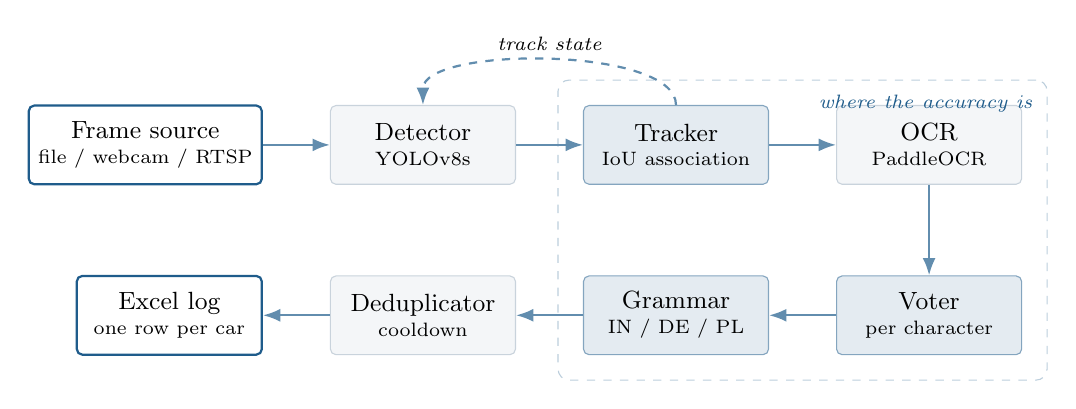
\begin{tikzpicture}[
  node distance=0.55cm and 0.85cm,
  box/.style={rectangle, rounded corners=2pt, draw=rule, fill=soft,
              minimum height=1.0cm, minimum width=2.35cm, align=center,
              font=\small},
  hl/.style={box, fill=accent!12, draw=accent!55},
  io/.style={box, fill=white, draw=accent, thick},
  arr/.style={-{Latex[length=2.2mm]}, draw=accent!70, thick},
]

\node[io]  (src)   {Frame source\\[-2pt]{\scriptsize file / webcam / RTSP}};
\node[box, right=of src] (det) {Detector\\[-2pt]{\scriptsize YOLOv8s}};
\node[hl,  right=of det] (trk) {Tracker\\[-2pt]{\scriptsize IoU association}};
\node[box, right=of trk] (ocr) {OCR\\[-2pt]{\scriptsize PaddleOCR}};

\node[hl,  below=1.15cm of ocr] (vote) {Voter\\[-2pt]{\scriptsize per character}};
\node[hl,  left=of vote]  (gram) {Grammar\\[-2pt]{\scriptsize IN / DE / PL}};
\node[box, left=of gram]  (dedup){Deduplicator\\[-2pt]{\scriptsize cooldown}};
\node[io,  left=of dedup] (xl)   {Excel log\\[-2pt]{\scriptsize one row per car}};

\draw[arr] (src) -- (det);
\draw[arr] (det) -- (trk);
\draw[arr] (trk) -- (ocr);
\draw[arr] (ocr) -- (vote);
\draw[arr] (vote) -- (gram);
\draw[arr] (gram) -- (dedup);
\draw[arr] (dedup) -- (xl);

\draw[arr, dashed] (trk.north) .. controls +(0,0.75) and +(0,0.75) .. (det.north)
  node[midway, above, font=\scriptsize\itshape] {track state};

\begin{scope}[on background layer]
  \node[draw=accent!30, dashed, rounded corners, fit=(trk)(vote)(gram),
        inner sep=9pt] (grp) {};
\end{scope}
\node[font=\scriptsize\itshape\color{accent}, anchor=north east]
      at ($(grp.north east)+(-2pt,-2pt)$) {where the accuracy is};
\end{tikzpicture}
\end{center}

The three highlighted stages are worth more than the model choices around them.
Tracking converts per-frame detections into vehicles; voting converts unreliable
readings into one answer; the grammar decides what is plausible. Section
\ref{sec:metrics} quantifies each.

\subsection{Module map}

\begin{center}
\small
\begin{tabular}{@{}llr@{}}
\toprule
\textbf{Module} & \textbf{Responsibility} & \textbf{Lines} \\
\midrule
\texttt{alpr.sources}   & Video files, webcams, RTSP; frame dropping    & 346 \\
\texttt{alpr.detect}    & Detector inference, device selection          & 194 \\
\texttt{alpr.track}     & IoU tracking, track lifecycle                 & 207 \\
\texttt{alpr.ocr}       & Plate crops, preprocessing, recognition       & 274 \\
\texttt{alpr.vote}      & Per-character multi-frame voting              & 186 \\
\texttt{alpr.plates}    & India, Germany, Poland grammars; correction   & 662 \\
\texttt{alpr.dedup}     & Cross-pass duplicate suppression              & 122 \\
\texttt{alpr.excel}     & Crash-safe workbook writing                   & 341 \\
\texttt{alpr.pipeline}  & Orchestration of all of the above             & 250 \\
\texttt{alpr.data}      & Dataset ingest, splitting, export             & 800 \\
\texttt{alpr.evaluate}  & Detection metrics, size slices, galleries     & 322 \\
\texttt{alpr.endtoend}  & End-to-end scoring, failure attribution       & 247 \\
\texttt{alpr.cer}       & Character error rate, ablation harness        & 189 \\
\texttt{alpr.dupes}     & Perceptual near-duplicate detection           & 286 \\
\texttt{alpr.viewer}    & Annotated video and live window               & 235 \\
\bottomrule
\end{tabular}
\end{center}

\newpage
% =================================================================== data ===
\section{Data}

\subsection{Sources}

The dataset is assembled from two openly licensed Roboflow Universe datasets,
both \textbf{CC BY 4.0}, which permits redistribution with attribution:

\begin{center}
\small
\begin{tabular}{@{}llr@{}}
\toprule
\textbf{Source} & \textbf{Content} & \textbf{Images} \\
\midrule
\texttt{e-hh49k/european-license-plates-tjviy} & European plates & 1{,}455 \\
\texttt{nivu/indian-license-plate-knte7}       & Indian plates   & 1{,}650 \\
\midrule
\multicolumn{2}{@{}l}{\textbf{Total}} & \textbf{3{,}105} \\
\bottomrule
\end{tabular}
\end{center}

Licence is treated as data, not documentation: each ingested record carries a
\texttt{source} tag, and the publishing step filters on it. A \texttt{NoDerivatives}
licence forbids publishing a re-split, which is precisely what this pipeline
produces, so such a source could be used locally but never redistributed.

\subsection{Splitting}

The dataset is split 2174 / 466 / 465 with three properties, each defending
against a specific way results can be inflated.

\begin{description}[leftmargin=1.2cm, style=nextline]
  \item[Grouped] Frames sampled from one video are near-duplicates. A per-image
    split places frame 100 in train and frame 101 in validation, so the model is
    evaluated on images it has effectively memorised. Everything sharing a group
    key goes to one split.
  \item[Stratified by region] With two regions in one dataset, an unlucky split
    can leave the test set almost entirely Indian, resting the European figure on
    a handful of images.
  \item[Deterministic] Assignment derives from \texttt{blake2b} of the group key
    rather than Python's \texttt{hash()}, which is salted per process and would
    produce a different split in a notebook than in CI.
\end{description}

The upstream train/validation/test split is discarded deliberately: it is random
per image, so near-duplicate shots of one scene straddle it.

\subsection{The leakage audit}
\label{sec:leakage}

Grouped splitting only catches what a filename admits to. Roboflow exports video
frames with names such as \texttt{dayride\_type1\_001-mp4-t-1062}, which the
grouping regular expression did not recognise as frames of one clip. A perceptual
hash audit (\texttt{alpr.dupes}) compared every image against every other:

\begin{center}
\small
\begin{tabular}{@{}lr@{}}
\toprule
Duplicate pairs found & 225 \\
Crossing a split boundary & 110 \\
Train $\leftrightarrow$ held-out (contaminating) & 102 \\
Test images with a twin in train & 27 (5.8\%) \\
\bottomrule
\end{tabular}
\end{center}

\keyfinding{%
\textbf{The leak did not carry the score.} Re-scoring the model on only the 438
uncontaminated test images changed recall by 0.0001 (0.9979 $\rightarrow$ 0.9978)
and \emph{improved} precision (0.9545 $\rightarrow$ 0.9556). The result stands,
and it stands with evidence rather than assumption. The grouping logic was
corrected so future splits cluster duplicates by perceptual hash, which catches
cases no filename convention would reveal.}

\newpage
% ============================================================== detection ===
\section{Detection}

\subsection{Training}

\begin{center}
\small
\begin{tabular}{@{}ll@{}}
\toprule
Architecture & YOLOv8s (11.1M parameters) \\
Epochs & 100 \\
Image size & 640 \\
Hardware & Google Colab T4, 1.25 hours \\
Reproducibility & config committed; run writes \texttt{provenance.json} \\
\bottomrule
\end{tabular}
\end{center}

Augmentation is where a general purpose recipe goes wrong for this object. A
plate is a small, rigid, text-bearing rectangle photographed from a camera above
bumper height:

\begin{center}
\small
\begin{tabular}{@{}llp{7.6cm}@{}}
\toprule
\textbf{Setting} & \textbf{Value} & \textbf{Reasoning} \\
\midrule
\texttt{flipud} & 0.0 & A plate is never upside down; vertical flips train an input that cannot occur. \\
\texttt{degrees} & 10 & Plates \emph{are} photographed rotated. Ultralytics defaults this to 0. \\
\texttt{perspective} & 0.0005 & And off-axis. Also defaults to 0. \\
\texttt{close\_mosaic} & 10 & Mosaic shrinks objects into the small-object regime; disabling it for the final epochs lets the model settle on undistorted images. \\
\bottomrule
\end{tabular}
\end{center}

\texttt{provenance.json} records the resolved configuration \emph{and the
Ultralytics version}, because that library changes augmentation defaults between
minor releases: a configuration alone does not pin a run.

\subsection{Results}

Measured on the held-out test split of 465 images the model never saw:

\begin{center}
\small
\begin{tabular}{@{}lr@{}}
\toprule
mAP@50 & \textbf{0.9921} \\
mAP@50--95 & 0.8377 \\
Precision & 0.9816 \\
Recall & \textbf{0.9917} \\
Inference (T4) & 4.7\,ms/image \\
Inference (Apple M4, MPS) & 29\,ms/frame \\
\bottomrule
\end{tabular}
\end{center}

\keyfinding{%
\textbf{Recall matters more than precision at this stage.} A plate the detector
misses can never be read downstream --- that error is unrecoverable. A false
positive produces a crop, OCR emits noise, and the grammar rejects it. The
observed error profile is the right way round: \textbf{1 missed plate against 23
false positives} across the entire test split.}

\subsection{Performance by plate size}

Aggregate metrics hide the population that matters. Precision and recall
bucketed by ground-truth plate width:

\begin{center}
\small
\begin{tabular}{@{}lrrr@{}}
\toprule
\textbf{Plate width} & \textbf{n} & \textbf{Precision} & \textbf{Recall} \\
\midrule
tiny ($<$32\,px)      & 8   & 1.0000 & 1.0000 \\
small (32--64\,px)    & 64  & 0.9000 & 0.9844 \\
medium (64--128\,px)  & 191 & 0.9598 & 1.0000 \\
large ($\geq$128\,px) & 190 & 0.9845 & 1.0000 \\
\bottomrule
\end{tabular}
\end{center}

Small plates were expected to cap end-to-end accuracy. They do not: every plate
under 32 pixels was found. The single miss sits in the 32--64\,px band.

\newpage
% ============================================================ recognition ===
\section{Recognition}

\subsection{Measuring at all}

Neither source dataset ships plate \emph{text}, only bounding boxes. Character
error rate therefore could not be measured without ground truth, so 124 test
crops were hand-labelled with a purpose-built tool (\texttt{alpr label}), sampled
across size buckets so the figure is not flattered by easy plates.

Character error rate is edit distance over reference length, aggregated across
the corpus rather than averaged per sample so one badly read short plate cannot
dominate:

\[
\mathrm{CER} = \frac{\sum_i \mathrm{lev}(r_i, h_i)}{\sum_i |r_i|}
\]

Exact-match accuracy is reported alongside it, because for a plate log that is
what actually matters: a plate with one wrong character is a wrong plate, not a
90\%-correct one.

\subsection{Preprocessing: a negative result}

The expectation was that upscaling small crops and normalising contrast would be
free accuracy --- crops are often 40\,px tall against a model trained on
$\approx$48\,px text. Measured against a control on the 124 labelled crops:

\begin{center}
\small
\begin{tabular}{@{}lrr@{}}
\toprule
\textbf{Variant} & \textbf{CER} & \textbf{Exact match} \\
\midrule
\textbf{raw (control)} & \textbf{0.2291} & 30.6\% \\
upscale only & 0.2301 & 29.8\% \\
grey + contrast & 0.2380 & 30.6\% \\
upscale + grey + contrast \textit{(former default)} & 0.2410 & 30.6\% \\
+ sharpen & 0.2500 & 27.4\% \\
\bottomrule
\end{tabular}
\end{center}

\keyfinding{%
\textbf{Every preprocessing step made accuracy worse, and the original default
was the second-worst configuration available.} PaddleOCR already resizes and
normalises each crop to its own input specification, so preprocessing first
resamples twice and destroys detail the model would otherwise have used. The
default was changed to apply nothing. An earlier ablation on \emph{synthetic}
renders had shown no effect either way; only real crops revealed the harm, which
is the argument for labelling real data rather than trusting a clean proxy.}

\subsection{What preprocessing cannot do}

Perspective correction requires the plate's four corners, and the detector emits
an axis-aligned box. Rotating by a guessed angle is as likely to hurt as help.
Genuine de-skew needs an oriented-bounding-box or segmentation model, which is a
change to the detector, not something preprocessing can fake.

\newpage
% ================================================================ grammar ===
\section{Plate grammars}

\subsection{Why grammar-constrained correction}

OCR confuses characters that look alike: \texttt{0/O}, \texttt{1/I}, \texttt{5/S},
\texttt{8/B}. Correcting these blindly makes accuracy \emph{worse}, because it
breaks every plate that legitimately contains a zero. Correcting them against a
\emph{grammar} is safe, because the grammar states which positions may hold a
letter and which a digit.

Correction is a bounded edit search rather than a positional rewrite, because
formats have variable-length parts: Germany's district prefix is one to three
letters, so position alone does not determine the character class. At most two
characters are reinterpreted; beyond that, a ``match'' says more about the search
than about the plate.

\subsection{Three grammars, three different strictness policies}

\begin{center}
\small
\begin{tabular}{@{}lp{10.6cm}@{}}
\toprule
\textbf{India} & \texttt{MH 12 AB 1234}: state code, district digits, optional
series letters, one to four digits. Unknown state codes lower confidence sharply,
because the list is closed in practice. \\[3pt]
\textbf{Germany} & \texttt{DA-XY 123}: district prefix, letters, digits, optional
\texttt{E}/\texttt{H} suffix, at most eight body characters. Unknown districts
are \emph{accepted} at reduced confidence --- roughly 700 exist and the set
changes. \\[3pt]
\textbf{Poland} & \texttt{PO 2427W}: territorial code plus a four or five
character series with at most two letters. \\
\bottomrule
\end{tabular}
\end{center}

\keyfinding{%
\textbf{Poland is the strongest grammar in the system, and the format explains
why.} Polish plates ban the letters \texttt{B}, \texttt{D}, \texttt{I},
\texttt{O} and \texttt{Z} from the series \emph{precisely because they resemble
digits}, and \texttt{Q} is absent from the language entirely. The ambiguity was
removed at the design stage, so a \texttt{B} in the series is not a probable
\texttt{8} --- it is a certain one. This is the clearest case in the project of a
real-world format encoding exactly the constraint an OCR pipeline needs.}

\subsection{Ambiguity that only context resolves}

\texttt{MAB123E} fits both \texttt{M-AB 123E} (München) and \texttt{MA-B 123E}
(Mannheim), and both prefixes are real. The string alone cannot settle it; the
hyphen that OCR read can. Normalisation strips separators, so the separator
position is captured \emph{before} normalisation runs and used to break the tie.

\subsection{Measured effect}

On the 124 labelled crops, comparing raw OCR output against grammar-corrected
output:

\begin{center}
\small
\begin{tabular}{@{}lrrrr@{}}
\toprule
 & \textbf{CER raw} & \textbf{CER + grammar} & \textbf{Exact raw} & \textbf{Exact + grammar} \\
\midrule
Overall (124) & 0.2291 & \textbf{0.1693} & 30.6\% & \textbf{43.5\%} \\
Indian (65)   & 0.2067 & \textbf{0.1138} & 36.9\% & \textbf{61.5\%} \\
European (59) & 0.2658 & 0.2605 & 23.7\% & 23.7\% \\
\bottomrule
\end{tabular}
\end{center}

\keyfinding{%
\textbf{Indian accuracy rises from 37\% to 62\%. European accuracy does not move
at all.} That is not a defect --- it is the method working and being limited by
scope. At that point the grammars modelled India and Germany, while the European
dataset is \emph{pan}-European. A grammar cannot correct toward a rule it does
not have. The honest generalisation is that grammar-constrained correction is
worth roughly \textbf{+25 accuracy points on formats you have modelled, and
nothing on formats you have not}.}

This finding directly motivated adding the Polish grammar; Section
\ref{sec:e2e} quantifies the result.

\newpage
% =============================================== tracking, voting, logging ===
\section{Tracking, voting and logging}

\subsection{Tracking}

Association is IoU-based rather than a Kalman filter. Plates move smoothly
between frames at any reasonable framerate, there is a single class, and plates
rarely occlude one another, so a motion model would not earn its complexity.

Two parameters carry most of the value:

\begin{description}[leftmargin=1.2cm, style=nextline]
  \item[\texttt{min\_hits}] A track must be seen this many times before it is
    confirmed. This is the single-frame false-positive filter, and it matters
    because that is exactly the detector's measured error profile: 23 false
    positives against 1 miss, most appearing in one frame only. A real plate
    persists; a spurious box on a headlight does not.
  \item[\texttt{max\_age}] How many frames a track survives unmatched. Plates
    disappear briefly behind wipers and other vehicles; killing a track on the
    first missed frame would log one vehicle twice.
\end{description}

\subsection{Voting is per character, not per string}

This is the design decision with the largest gap between the obvious approach and
the correct one. Consider one vehicle read across four frames:

\begin{center}
\small
\begin{tabular}{@{}ll@{}}
\toprule
\texttt{MH12AB1234} & correct \\
\texttt{MH12A81234} & \texttt{B} misread as \texttt{8} \\
\texttt{MH12AB1Z34} & \texttt{2} misread as \texttt{Z} \\
\texttt{NH12AB1234} & \texttt{M} misread as \texttt{N} \\
\bottomrule
\end{tabular}
\end{center}

No string holds a majority --- every read differs from every other. String-level
voting picks one arbitrarily and is right only by luck.

\keyfinding{%
\textbf{Per-character voting is correct at every position}, because each error
appears in a minority of frames and is outvoted. The result is a plate that
\emph{no single frame read correctly}. Reads are weighted by confidence, so a
crisp close-up outvotes a blurred distant one rather than merely being
outnumbered by it.}

Length is settled first, by confidence weight, because voting per position across
mixed-length reads smears characters into the wrong slots. Ties break
alphabetically: a nondeterministic plate would be worse than a wrong one.

\subsection{Logging}

An \texttt{.xlsx} workbook is a zip archive of XML, so adding a row means
rewriting the whole file. Saving after every plate rewrites it thousands of times
over one video; saving only at the end loses the entire run to a crash. Every
accepted event is therefore appended to a \textbf{JSONL write-ahead journal} the
instant it occurs, and the workbook is materialised from that journal. A run
interrupted at any point can be rebuilt with nothing lost, and a torn final line
--- the only line a crash can damage --- is skipped while mid-file corruption
still raises.

Deduplication here is \emph{cross-pass}, not within-pass: suppressing repeated
frames of one sighting is the tracker's job, while this handles the vehicle that
circles a car park and returns, which no tracker can suppress because the second
sighting genuinely is a new track.

\newpage
% ============================================================ end-to-end ===
\section{End-to-end evaluation}
\label{sec:e2e}

\subsection{Method}

The whole pipeline is run over the 124 labelled plates --- detect, crop, read,
validate --- and every plate is attributed to the stage that lost it. The
headline number alone does not say where to invest; the breakdown does.

\begin{center}
\small
\begin{tabular}{@{}lp{9.8cm}@{}}
\toprule
\texttt{CORRECT} & The pipeline produced exactly the right string. \\
\texttt{DETECTION\_MISS} & No box overlapped the plate; nothing downstream could help. \\
\texttt{OCR\_ERROR} & Found, read wrong, grammar could not repair it. \\
\texttt{GRAMMAR\_REJECTED} & The grammar refused the read, so nothing was logged. \\
\texttt{GRAMMAR\_CORRUPTED} & OCR was right and the grammar made it wrong. \\
\bottomrule
\end{tabular}
\end{center}

The final category is why the taxonomy exists. A correction step that damages
correct reads is worse than no correction step, and it is invisible in an
aggregate score because the losses sit inside the same number as the gains.

Precision and recall are deliberately asymmetric about rejection: a refused read
costs a plate (lowering recall) but does not put a wrong plate in the log (so it
does not lower precision). That is the grammar working rather than failing.

\subsection{Results}

\begin{center}
\small
\begin{tabular}{@{}lrr@{}}
\toprule
\textbf{Outcome} & \textbf{Count} & \textbf{Share} \\
\midrule
Correct & 72 & 58.1\% \\
\textbf{Detection miss} & \textbf{0} & \textbf{0\%} \\
Grammar rejected & 30 & 24.2\% \\
OCR error & 21 & 16.9\% \\
Grammar corrupted a correct read & 1 & 0.8\% \\
\midrule
\multicolumn{3}{@{}l}{End-to-end accuracy \textbf{58.1\%}, precision \textbf{76.6\%} of 94 logged} \\
\bottomrule
\end{tabular}
\end{center}

\keyfinding{%
\textbf{Detection lost nothing.} Not one of the 124 plates was missed, consistent
with the detector's 0.998 recall. Every remaining failure is a \emph{reading}
failure --- so additional detector training would buy exactly zero. This is the
single most actionable statement the evaluation produces, and an aggregate score
would have hidden it completely.}

\subsection{Adding one grammar outperformed any model change}

The first end-to-end run scored 42.7\%, with two thirds of European plates
\emph{refused rather than misread}. Modelling Poland followed directly from that
diagnosis. Neither the detector nor the OCR engine changed between these rows:

\begin{center}
\small
\begin{tabular}{@{}lrrrr@{}}
\toprule
\textbf{Grammars} & \textbf{End-to-end} & \textbf{European} & \textbf{Polish} & \textbf{Precision} \\
\midrule
India + Germany & 42.7\% & 15.3\% & --- & 71.6\% \\
+ Polish standard & 50.0\% & 30.5\% & 50.0\% & 71.3\% \\
+ Polish individual plates & \textbf{58.1\%} & \textbf{47.5\%} & \textbf{72.2\%} & \textbf{76.6\%} \\
\bottomrule
\end{tabular}
\end{center}

Precision rose alongside recall, which is unusual --- modelling a format properly
removes wrong ``corrections'' as well as adding right ones. Polish plates now
score higher than Indian ones, for the reason given in the grammar section.

\subsection{Two bugs found only by end-to-end measurement}

\begin{enumerate}[leftmargin=*]
  \item \textbf{Indian plates carry one to four trailing digits, not exactly
    four.} The grammar demanded four and silently rejected \texttt{KL54H369},
    \texttt{TN58AM1} and \texttt{KL7BZ99}, all genuine. The unit tests did not
    catch it because they were written from the same wrong assumption as the
    code. Loosening the rule recovered three plates at the cost of roughly two
    points of precision \emph{and} some correction power: \texttt{MH12ABB234} is
    now a legitimate reading, so the grammar no longer repairs that \texttt{B} as
    an \texttt{8}. Both halves of the trade are pinned by tests.
  \item \textbf{Polish vanity plates were being corrupted into standard ones.}
    Every corrupted read was a one-letter plate that a \emph{single} edit pushed
    into the two-letter standard shape (\texttt{P74103} $\rightarrow$
    \texttt{PT4103}). Modelling individual plates at lower confidence makes the
    exact reading win; corruptions fell from three to one.
\end{enumerate}

\newpage
% =========================================================== live operation ===
\section{Live operation}

\subsection{Files and cameras fail in opposite directions}

A file is offline: every frame matters, and falling behind costs only time. A
camera is live, and the enemy is \emph{latency}. OpenCV buffers frames, so if
detection takes 60\,ms while the camera produces one every 33\,ms, the buffer
fills and each frame read is older than the last --- seconds behind reality
within a minute, with no recovery.

\keyfinding{%
The fix is not to run faster but to \textbf{throw frames away}. A reader thread
consumes the camera continuously and keeps only the newest frame, so the pipeline
always processes what the camera sees \emph{now}. Dropping frames on a file would
silently discard \emph{data}; keeping them on a camera silently discards
\emph{time}.}

RTSP adds reconnection with exponential backoff, because a source that dies on
the first network interruption makes an unattended camera useless.

\subsection{Throughput}

Measured end to end on an Apple M4, detection on Metal (MPS) and recognition on
CPU:

\begin{center}
\small
\begin{tabular}{@{}lr@{}}
\toprule
Detection & 34.6\,fps (29\,ms/frame) \\
OCR per plate crop & 41.1\,ms \\
Full pipeline, \texttt{ocr\_every}\,=\,1 & 14.3\,fps \\
Full pipeline, \texttt{ocr\_every}\,=\,3 & \textbf{23.5\,fps} \\
\bottomrule
\end{tabular}
\end{center}

\keyfinding{%
\textbf{Recognition costs more than detection} --- 41\,ms against 29\,ms. The
``small'' stage is the bottleneck. Reading every frame misses a 15\,fps target
while reading every third frame clears it comfortably, and a track does not need
forty reads: voting is decisive with a handful.}

\newpage
% =========================================================== requirements ===
\section{Requirements}

\subsection{Software}

\begin{center}
\small
\begin{tabular}{@{}lll@{}}
\toprule
\textbf{Package} & \textbf{Version} & \textbf{Role} \\
\midrule
Python & $\geq$3.11 & Runtime \\
\texttt{ultralytics} & $\geq$8.3 & YOLO training and inference \\
\texttt{opencv-python-headless} & $\geq$4.10 & Video I/O, drawing \\
\texttt{pillow} & $\geq$10.0 & Image handling, header-only size reads \\
\texttt{openpyxl} & $\geq$3.1 & Excel writing \\
\texttt{numpy}, \texttt{pandas}, \texttt{pyyaml} & --- & Support \\
\midrule
\multicolumn{3}{@{}l}{\textit{Optional extra} \texttt{[ocr]}} \\
\texttt{paddlepaddle} & $\geq$3.3 & OCR backend (CPU) \\
\texttt{paddleocr} & $\geq$3.7 & Text recognition \\
\midrule
\multicolumn{3}{@{}l}{\textit{Optional extra} \texttt{[dev]}: pytest, ruff, pre-commit, nbstripout} \\
\bottomrule
\end{tabular}
\end{center}

The OCR stack is a separate extra because nothing before the recognition stage
imports it, and because it carries a subtlety worth recording: only
\texttt{paddlepaddle-gpu} is frozen at an old version with no macOS wheel. The
\emph{CPU} build ships current wheels for all supported Python versions on macOS
arm64, Linux and Windows. CPU is also the right default regardless of hardware,
because recognition runs on a crop of a few thousand pixels and the GPU has
almost nothing to accelerate.

\subsection{Hardware}

\begin{center}
\small
\begin{tabular}{@{}lll@{}}
\toprule
\textbf{Task} & \textbf{Minimum} & \textbf{Used here} \\
\midrule
Training & CUDA GPU & Colab T4 (16\,GB), 1.25\,h \\
Inference (batch) & CPU & Apple M4 via MPS \\
Inference (live) & CPU, GPU recommended & Apple M4, 23.5\,fps \\
Dataset storage & $\approx$110\,MB & External SSD \\
\bottomrule
\end{tabular}
\end{center}

Training deliberately targets a free Colab T4. That constrains the design in one
important way: the free tier grants a single session and its filesystem does not
survive it, so every notebook must be able to rebuild whatever it needs rather
than depending on a previous notebook's output.

\subsection{Credentials}

No credential is ever stored in source, in a notebook cell, or in a
configuration file. Keys are read from the environment or from the notebook
platform's secret store, and a missing key raises with instructions rather than
silently falling back. Two automated safeguards enforce this: a \texttt{gitleaks}
pre-commit hook, and a CI test that fails if any notebook contains a
credential-shaped token.

\newpage
% ================================================================= CI/CD ===
\section{Continuous integration}

\subsection{Configuration}

\begin{lstlisting}[language=bash, caption={\texttt{.github/workflows/ci.yml}}]
name: CI

on:
  push:
    branches: ["**"]
  pull_request:
    branches: [main]

jobs:
  test:
    runs-on: ubuntu-latest
    steps:
      - uses: actions/checkout@v5
      - uses: actions/setup-python@v6
        with:
          python-version: "3.12"
          cache: pip

      - name: Install
        run: pip install -e ".[dev]"

      - name: Lint
        run: |
          ruff check .
          ruff format --check .

      - name: Test
        run: pytest
\end{lstlisting}

CI runs on \emph{every} branch, not only pull requests, so a mistake is caught
before review rather than during it. The OCR extra is deliberately not installed:
the runner has no GPU, and the tests that would exercise it are opt-in anyway.

\subsection{Test strategy}

577 tests run in CI without a GPU, a camera, or model weights. Tests requiring
those are marked and skipped by default:

\begin{center}
\small
\begin{tabular}{@{}ll@{}}
\toprule
\texttt{pytest -m gpu} & Requires CUDA \\
\texttt{pytest -m weights} & Requires trained weights or a downloaded model \\
\texttt{pytest -m camera} & Requires a webcam or reachable stream \\
\bottomrule
\end{tabular}
\end{center}

The principle is that a suite nobody can run green is a suite nobody runs. Heavy
dependencies are stubbed at the boundary, so what is tested is the project's own
logic --- matching, voting, splitting, attribution --- rather than whether YOLO
or PaddleOCR work.

\subsection{Guards against silent regressions}

Notebooks are the weak point in any repository like this, because saving one from
a hosted platform writes straight to the default branch and bypasses pre-commit
entirely. A dedicated test asserts, for every committed notebook: valid JSON, no
saved cell outputs, no install of a removed dependency extra, and no
credential-shaped token. This is not hypothetical --- it caught a dependency fix
being silently reverted twice, and cell outputs being committed once.

\subsection{Development workflow}

\begin{enumerate}[leftmargin=*]
  \item Branch per change; the default branch is never committed to directly.
  \item Push triggers CI: lint, format check, full suite.
  \item Pull request with the reasoning, not just the diff --- specifically what
        was measured and what the measurement said.
  \item Merge only on green.
\end{enumerate}

\newpage
% ============================================================== metrics ===
\section{Consolidated performance metrics}
\label{sec:metrics}

\begin{center}
\small
\begin{longtable}{@{}llr@{}}
\toprule
\textbf{Stage} & \textbf{Metric} & \textbf{Value} \\
\midrule
\endhead
Detection & mAP@50 (test) & 0.9921 \\
Detection & mAP@50--95 (test) & 0.8377 \\
Detection & Precision & 0.9816 \\
Detection & Recall & 0.9917 \\
Detection & Missed plates (465 images) & 1 \\
Detection & False positives & 23 \\
\midrule
OCR (GT crops) & CER, raw & 0.2291 \\
OCR (GT crops) & CER, grammar-corrected & 0.1693 \\
OCR (GT crops) & Exact match, raw & 30.6\% \\
OCR (GT crops) & Exact match, corrected & 43.5\% \\
\midrule
End-to-end & Accuracy & 58.1\% \\
End-to-end & Precision & 76.6\% \\
End-to-end & Detection misses & 0 \\
End-to-end & Indian accuracy & 67.7\% \\
End-to-end & European accuracy & 47.5\% \\
End-to-end & Polish accuracy & 72.2\% \\
\midrule
Throughput & Detection (M4, MPS) & 34.6\,fps \\
Throughput & OCR per crop (CPU) & 41.1\,ms \\
Throughput & Full pipeline (\texttt{ocr\_every}=3) & 23.5\,fps \\
\midrule
Data & Images / plates & 3{,}105 / 3{,}273 \\
Data & Split (train/val/test) & 2174 / 466 / 465 \\
Data & Hand-labelled for OCR & 124 \\
\midrule
Code & Tests & 577 \\
Code & Source lines & $\approx$6{,}500 \\
\bottomrule
\end{longtable}
\end{center}

\section{Limitations}

Stated plainly, because a documented limitation is worth more than an
undocumented strength.

\begin{enumerate}[leftmargin=*]
  \item \textbf{Region labels can be wrong where formats overlap.} Romanian
    plates satisfy the Polish grammar. The text is read correctly; the region
    column says \texttt{PL} where it should say \texttt{RO}.
  \item \textbf{Only three grammars exist.} Plates from unmodelled countries are
    refused rather than misread --- safe, but it caps recall.
  \item \textbf{No perspective correction.} The detector emits axis-aligned
    boxes, so obliquely photographed plates are read as-is.
  \item \textbf{mAP was not recomputed on the leak-free subset.} The audit
    compared precision and recall at a fixed confidence threshold, not the
    precision--recall curve integral.
  \item \textbf{The OCR figures rest on 124 labels.} Enough for the effects
    observed, which are large, but not for fine distinctions.
  \item \textbf{Plate data is personal data.} Under the GDPR and comparable
    regimes, deploying this against public traffic engages obligations around
    lawful basis, retention and notice. Labelled crops and transcriptions are
    deliberately excluded from version control for this reason.
\end{enumerate}

\newpage
% ============================================================== interview ===
\section{Interview questions and answers}

\subsection*{Architecture and design}

\paragraph{Q1. Walk me through the system.}
Frames arrive from a file, webcam or RTSP stream. A YOLOv8s detector finds plates
per frame. An IoU tracker assigns each plate a stable identity across frames, so
one vehicle is one track rather than forty detections. Every few frames the
track's best crop is read by OCR, and the readings accumulate. When the track
ends, the readings are voted into a single string per character, that string is
validated against a country plate grammar, and the survivor is written as one row
in an Excel workbook. A cooldown suppresses the same plate reappearing minutes
later.

\paragraph{Q2. Why track at all? Why not read every frame independently?}
Two reasons. First, the output would be unusable: one car produces forty rows.
Second, and more importantly, tracking is what makes voting possible, and voting
is where a large part of the accuracy comes from. It also acts as a
false-positive filter --- requiring a track to persist for several frames before
it is confirmed eliminates spurious single-frame detections, which is precisely
this detector's error profile.

\paragraph{Q3. Why per-character voting rather than majority voting on strings?}
Because in real data no string usually holds a majority. In one measured example
four reads of the same plate were all different, and the correct string appeared
once while a wrong one appeared twice --- string voting picks the wrong answer.
Per-character voting is right at each position because each error appears in a
minority of frames, and it can produce a plate that no single frame read
correctly.

\paragraph{Q4. Why not use ByteTrack, which ships with Ultralytics?}
Using it means driving detection through Ultralytics' tracking API, which couples
the whole pipeline to that library. The tracking problem here is also easy:
smooth motion, one class, little occlusion. IoU association gives the same result
for a fraction of the complexity, and the pipeline keeps its own detection type.

\subsection*{Data and evaluation}

\paragraph{Q5. How do you know your test score is not inflated?}
I audited for it. A perceptual hash comparison found that 5.8\% of test images had
a near-duplicate in training --- consecutive video frames the grouping logic did
not recognise. Re-scoring on the uncontaminated subset moved recall by 0.0001, so
the leak was not carrying the score, and I fixed the grouping so future splits
cluster duplicates by image content rather than by filename.

\paragraph{Q6. Why is your split grouped and stratified?}
Grouped because frames from one video are near-duplicates: a per-image split
evaluates the model on pictures it has memorised. Stratified because with two
regions in one dataset an unlucky split can leave the test set almost entirely
one region, so the other region's number rests on a handful of images. And
deterministic via \texttt{blake2b} rather than Python's \texttt{hash()}, which is
salted per process and would differ between a notebook and CI.

\paragraph{Q7. Your detector scores 0.99 mAP. Is that not suspiciously high?}
It is high, which is why I checked it rather than reporting it. Plate detection is
an easy task --- a high-contrast rectangle of near-fixed aspect ratio on a vehicle
--- and published detectors land in this range. The leakage audit ruled out the
obvious alternative explanation. The more informative number is that end-to-end
accuracy is 58\%: the detector is not the hard part.

\paragraph{Q8. Why report a failure breakdown rather than a single accuracy?}
Because the breakdown says what to do next and the aggregate does not. Mine shows
zero detection misses, which means further detector training would buy nothing,
and that the dominant loss is grammar rejection on unmodelled plate formats. That
directly produced the next change and a 15-point improvement.

\subsection*{Judgement}

\paragraph{Q9. Tell me about something you got wrong.}
I assumed preprocessing crops --- upscaling, contrast normalisation --- would
improve OCR, and made it the default. Measured against a control on labelled
data, every step made accuracy \emph{worse}, and my default was the second-worst
configuration available. PaddleOCR normalises crops internally, so preprocessing
first resamples twice and destroys detail. I removed it. An earlier test on
synthetic images had shown no effect; only real crops showed the harm.

\paragraph{Q10. Give an example of a bug your tests could not catch.}
My Indian grammar required exactly four trailing digits. Real plates carry one to
four, so it silently rejected valid plates. The unit tests passed because I had
written them from the same wrong assumption as the code --- the fixture plates
all had four digits. Only labelled real data exposed it. That is the argument for
evaluating against ground truth rather than against your own expectations.

\paragraph{Q11. What was the highest-leverage change you made?}
Adding a Polish plate grammar. The failure breakdown showed two thirds of
European plates were refused rather than misread, because the grammars covered
India and Germany while the data was pan-European. Adding Poland moved end-to-end
accuracy from 42.7\% to 58.1\% and raised precision at the same time. No model
was retrained.

\paragraph{Q12. Why does correcting OCR against a grammar work?}
Because it converts an ambiguous decision into a constrained one. OCR confuses
\texttt{0/O} and \texttt{8/B}; correcting blindly damages every plate that
legitimately contains a zero. A grammar states which positions hold digits, so
only genuinely impossible characters are changed. Poland is the extreme case: its
format bans exactly the confusable letters from the series, so a \texttt{B} there
is not a probable \texttt{8} but a certain one.

\paragraph{Q13. Where does this system fail, and what would you do about it?}
Formats it does not model. Romanian plates satisfy the Polish grammar, so the
text is right but the region label is wrong; unmodelled countries are refused
entirely. The fix is more grammars, which is cheap --- the interface is small and
has three implementations to copy. Beyond that, oblique plates cannot be
de-skewed because the detector emits axis-aligned boxes; that needs an
oriented-box model, which is a detector change rather than a post-processing one.

\subsection*{Engineering}

\paragraph{Q14. How do you keep a live camera from falling behind?}
By discarding frames. OpenCV buffers, so a pipeline slower than the camera reads
progressively staler frames and never recovers. A reader thread consumes the
camera continuously and retains only the newest frame. Dropping frames on a
\emph{file} would discard data, so file sources are not threaded --- the two
cases fail in opposite directions and are separate classes.

\paragraph{Q15. Why a write-ahead journal for an Excel file?}
Because \texttt{.xlsx} is a zip of XML: adding a row rewrites the whole archive.
Saving per plate is prohibitively slow and saving only at the end loses
everything to a crash. Each event is appended to a JSONL journal immediately and
the workbook is materialised from it, so an interrupted run can be rebuilt
completely.

\paragraph{Q16. Why is OCR not run on every frame?}
Because it is the bottleneck --- 41\,ms per crop against 29\,ms for detection.
Reading every frame yields 14.3\,fps, below a 15\,fps target; reading every third
frame yields 23.5\,fps. A track does not need forty readings for the vote to be
decisive.

\paragraph{Q17. How do you handle credentials?}
They never enter source, notebooks or configuration. They are read from the
environment or the platform secret store, and a missing key raises with
instructions rather than falling back to a default. A \texttt{gitleaks}
pre-commit hook and a CI test that rejects credential-shaped tokens in notebooks
enforce it, because the repository is public and anything pushed must be treated
as permanently disclosed.

\paragraph{Q18. What would you do differently with more time?}
Label more data --- 124 plates supports the large effects observed but not fine
distinctions. Add grammars for the remaining European formats. Train an
oriented-bounding-box detector so oblique plates can be de-skewed before
recognition. And measure the tracker directly against a video with a known
vehicle count; at present its contribution is inferred from the end-to-end
number rather than isolated.

\vfill
\begin{center}
\small\color{accent}
\rule{0.35\linewidth}{0.4pt}\\[0.4em]
Every figure in this document was produced by running the system.\\
Where a measurement contradicted the design, the design changed.
\end{center}

\end{document}
